%=========================================================================
% 
\chapter{System for streaming multimedia data from Android devices}
\label{chap:chapter5}
The previous chapters described important parts of the Android IP camera system from a theoretical point of view. This chapter concentrates on the design and implementation details of the resultant system, which consists of application server and Android application.

System requirements are analysed at the beginning followed by the system architecture and component implementation details.  Communication, Google Cloud Messaging, libraries used and user interface design are in the second part of this section.

The project is maintained on GitHub repository\footnote{Android IP camera GitHub repository: \url{https://github.com/JanChvala/thesis-ipcam}} and I hope I will be able to implement the feature ides in near future.


\section{Requirements}
The goal is to create a system which allows a user to stream video from Android device and play this video in the web browser. The video stream should be started only when it is requested and it should be possible even if the device is hidden behind NAT. The stream will be broadcast so it is important not to request the user media from the user who wants to playback the stream. The application has to provide usable user interface and basic stream settings and password protection.\\

\noindent
\textbf{Android application has to:}\vspace{-0.3em}
\begin{itemize}
	\item be able to get a stream from camera,
	\item start a stream when requested,
	\item have simple user interface,
	\item protect a stream with password,
	\item allow to change stream properties.
\end{itemize}

\newpage
\noindent
\textbf{Application server has to:}\vspace{-0.5em}
\begin{itemize}
	\item be able to process requests for a stream,
	\item show the requested stream to a user,
	\item have simple user interface,
	\item set a password for the stream.
\end{itemize}

These requirements are fulfilled and implemented as described in the next sections.

\section{System architecture design}
The system architecture consists of the application server and Android application. Handling push notifications\footnote{Simple messages which are sent (pushed) from the server to the client application.} also requires GCM servers (see chapter \ref{chap:chapter4}) to be involved and WebRTC requires signalling servers to establish direct communication between peers\footnote{Default signalling servers for RTCMultiConnection library are \url{http://firebase.io}.}.

The whole system overview with all its components can be seen in figure \ref{fig:implArchitecture}.

\insertImg[0.97]{impl-architecture.pdf}{Android IP camera system architecture.}{fig:implArchitecture}

\subsection{Application server}
The application server is responsible for serving static HTML files {streaming HTML page and playback HTML page}, handling client application registration (using simple REST\footnote{Representational State Transfer.} API) and sending GCM messages to a client.\\

\newpage
\noindent
Server back--end\footnote{Implementation of database, REST API and sending GCM messages.} is implemented with Node.js framework and these libraries:
\begin{itemize}
	\item \textbf{Node.js} - Platform built on top of Chrome's JavaScript runtime.
	\item \textbf{express\footnote{express: \url{http://expressjs.com/}}} - Minimalist web framework for server core functionality and routing.
	\item \textbf{node-gcm\footnote{node-gcm: \url{https://github.com/ToothlessGear/node-gcm}}} - Node.js library for handling Google Cloud Messaging.
	\item \textbf{passport\footnote{passport: \url{http://passportjs.org/}}} - Node.js library used for HTTP request authentication.
	\item \textbf{mongoose\footnote{mongoose: \url{http://mongoosejs.com/}}} - Node.js library used for working with MongoDB.
\end{itemize}



\noindent
Front--end is implemented using these technologies:
\begin{itemize}
	\item \textbf{HTML 5} - HyperText Markup Language - standard markup language for creating web pages.
	\item \textbf{CSS 3.0} - Cascading Style Sheets - handles the visual style of web page written in markup language.
	\item \textbf{AngularJS 1.4} - JavaScript web application framework.
	\item \textbf{RTCMultiConnection.js} - WebRTC library for JavaScript.
	\item \textbf{firabase.js} - JavaScript library used for WebRTC signalling.
\end{itemize}


The core of the front--end application was generated with Yeoman\footnote{Scaffolding tool for web applications. \url{http://www.yeoman.io}.} and its gulp-angular\footnote{The gulp-angular generator creates AngularJS base project with configured Gulp build system.} generator. These tools do more than just generating the structured base application but also provide more features such as ready--to--use development server or minification and code obfuscation for production build.

The application server implementation is important for the ability to start the stream when it is requested. It was developed using WebStorm IDE with student licence.




\subsection{Android application}
Client application for streaming the data from Android device is implemented in Java and runnable on Android version 4 (Ice Cream Sandwich) and above.

When running on Android 5 (Lollipop) and above the WebRTC is handled inside the application using native WebView component but the lack of native WebRTC support in WebView component prior to Lollipop versions puts restrictions to the resultant application. On Android 4 we use external web browser to handle the WebRTC. It is up to the user to choose which browser will handle the Intent. Chrome 42.02311 and Firefox 38.0.0 were tested as a compliant web browser capable of WebRTC.

WebRTC is crucial technology for the resultant system and cannot work without it. Using the demo application puts more restrictions and usability issues but it is working as expected.\\

\noindent
Implementation is dependent on the following libraries:
\begin{itemize}
	\item \textbf{Google Play Services} - The important module of Google Play Services is the \textit{play--services-gcm}\footnote{Google Play Services setup: \url{http://developer.android.com/google/play-services/setup.html}.} which provides the ability to work with GCM services.
	\item \textbf{AndroidAnnotations\footnote{AndroidAnnotations library: \url{http://androidannotations.org/}}} - Open--source framework for speeding--up Android application development by generating boilerplate parts using a custom Java preprocessor.
	\item \textbf{Support libraries} - Libraries providing back--port compatibility and additional utility classes.
	\item \textbf{StandOut\footnote{StandOut library: \url{https://github.com/sherpya/StandOut/}}} - Library for creating floating UI elements using service.
	\item \textbf{Retrofit\footnote{Retrofit library: \url{http://square.github.io/retrofit/}}} - Library used for creating REST API clients from Java interfaces.
	\item \textbf{Material dialogs\footnote{Material dialogs: \url{https://github.com/afollestad/material-dialogs}}} - Implementation of Android dialogs with respect to Material Design guidelines.
	\item \textbf{Material\footnote{Material: \url{https://github.com/rey5137/material}}} - Implementation of Material Design components for Android.
\end{itemize}

Android Studio 1.2 together with Gradle 2.3 and Android SDK Build-tools 22.0.1 served as the base of the development environment.




\section{Application server capabilities and implementation}
This section describes individual parts of the application server and their implementation in more detail. The beginning focuses on the database and REST API. The end of this section describes the RTCMultiConnection JavaScript library and then it presents some parts of source code and UI of streaming and playback pages.

\subsection{Database}
There are barely any requirements for the database so it does not matter what database is used for such simple usage. We use MongoDB\footnote{MongoDB: \url{https://www.mongodb.org/}} which is NoSQL document--oriented database. The advantage is that we can work with object models. We work with \textit{mongoose} library for \textit{Node.js}.\\

\noindent
Device object model definition:\vspace{-0.5em}
\begin{lstlisting}
// loading mongoose library
var mongoose = require('mongoose'); 

// Define our device schema
var DeviceSchema = new mongoose.Schema({
    name: String,
    code: String,
    gcmRegistrationId: String,
    lastUpdate: Date
});
\end{lstlisting}

\noindent
Saving device into database:\vspace{-0.5em}
\begin{lstlisting}
// create new instance of device
var device = new Device();

// TODO: edit device properties

// Saving the device into database
device.save(function (err) {
  // handle error or do something on success
});
\end{lstlisting}

\noindent
Finding device by its code:\vspace{-0.5em}
\begin{lstlisting}
Device.find({code: deviceCode}, function (err, devices) {
  // handle errors or do something with device
});
\end{lstlisting}



\subsection{Representational State Transfer API}
The application server provides simple REST API. It allows to register Android application after successful registration to Google Cloud Messaging servers. It also provides endpoint for starting registered device using Google Cloud Messaging service.

\subsubsection{POST /api/devices}
This request registers device. It expects the body of the request to be this JSON object:

\begin{lstlisting}
{
  name: String,
  gcmRegistrationId: String 
}
\end{lstlisting}

\noindent
Server takes the property \verb!name! and \verb!gcmRegistrationId! and creates a new object representing the device:

\begin{lstlisting}
{
  name: String,
  gcmRegistrationId: String,
  code: String,
  lastUpdate: Date
}
\end{lstlisting}

Object's property \verb!lastUpdate! is filled with actual date of registration and value of property \verb!code! is generated pseudo random string with eight characters.


\subsubsection{GET /devices/:device-code/start--stream}
\label{sssec:rest-stream}
This request is used to start streaming from device with specific \verb!:device-code! code. When this request is invoked then the application server tries to find device by its code in the database. Then it sends a message to the device using the \verb!gcmRegistrationId! token.

This request is invoked using jQuery\footnote{jQuery is JavaScript framework: \url{https://jquery.com/}} from within the playback page.
\begin{lstlisting}
$.get("/api/devices/" + deviceCode + "/start-stream",
  function(response) {
    console.log(response);
  }
);
\end{lstlisting}



\subsection{RTCMultiConnection}
RTCMultiConnection\footnote{Muaz Khan - RTCMultiConnection: \url{http://www.rtcmulticonnection.org/}} is open--sourced library developed under MIT license\footnote{MIT license in Open source initiative: \url{http://opensource.org/licenses/MIT}}. It is wrapping RTCPeerConnection JavaScript API (from the same developer) which handles the Peer Connection establishment and provides many features which make the development with WebRTC easier.

We use this library for WebRTC session initiation, acquiring local media stream, joining the created session and transferring the stream using Peer connection. This library also handles signalling by default\footnote{RTCMultiConnection uses Firebase servers for signalling by default: \url{http://firebase.com}.} so we do not need to manage additional servers. 

\subsubsection{Channels and rooms}
It uses a simple concept of virtual channels with rooms. A channel is the main container for rooms which are represented as sessions. There can be multiple sessions in the same channel. Each session has its initiator (the peer who opened the room) and participants (who joined the room). Channels, rooms and peers have their own unique identifiers.


\begin{lstlisting}
// including library
<script src="//cdn.webrtc-experiment.com/RTCMultiConnection.js">
</script>

// signalling library
<script src="//cdn.webrtc-experiment.com/firebase.js"></script>

// joining the room with roomID this is inside script tag
var connection = new RTCMultiConnection(roomID);
\end{lstlisting}

For our purposes, the channel is unique for every device and contains only one room. Both channel and room identifiers are based on device hash which is generated on the server side. The streaming device is in the role of an initiator and the clients which play the stream are participants.


\subsubsection{Session connection constraints}
Session connection is affected by media constraints. There is one option in RTCMultiConnection library which does not occur in WebRTC specification -- boolean constraint \verb!oneway!. This property allows peers that only want to playback the stream not to be prompted with local media permission because the local media is never demanded. This option is very useful in our case for broadcasting the stream.

\begin{lstlisting}
// setting the session for video only
connection.session = {
  audio: false,
  video: true,
  oneway: false
};
...
// example of setting FullHD resolution
connection.media.min(1920, 1080);
connection.media.max(1920, 1080);
\end{lstlisting}

\subsubsection{Local media resolution}
Dealing with resolution can be a little tricky when working with WebRTC. There are three parameters for \verb!getLocalMedia()! function which affect the actual quality of video that is being transmitted. There are \verb!resolution!, \verb!frameRate! and \verb!bandwith!. All those attributes are the base values for codec settings.

Resolution is the most tricky one. The parameter is used only for initial settings for video source (e.g. front facing camera) to provide media with that particular resolution. This value is unchangeable in the future for the same session. A new session has to be created in case of the need for resolution to be changed. The \verb!frameRate! is self--explaining --- It is the number of frames per seconds which should be transmitted. Finally, it is the bandwidth. It is the limitation for network usage for this specific stream.

These attributes put demands on the codec which, in case of WebRTC, is the VP8\footnote{More information about VP8 codec can be found on the WebM project page: \url{http://www.webmproject.org/}} open--sourced codec. It tries to maximize the quality of transmitted media while keeping considerable bandwidth. This is harder for rapidly changing scenes rather than for static ones. WebRTC is trying to keep the frame rate so it sacrifices the resolution of the video during the streaming to satisfy the frame rate and bandwidth. This is noticeable and could be a limitation for some use cases when the resolution prioritizes over the frame rate.


\subsubsection{Working with session}
Both peers, the one who streams and the one who wants to play the stream, connect to the signalling channel. We could omit this for participants and simply joint the session but they would not get notified when a new session is ready and it would not be possible to distinguish whether the session exists or not. Connecting to the signal brings the ability to hook up to \verb!onNewSession! which is fired when a participant is connected to signalling channel and the initiator opens the session.

\begin{lstlisting}
// all users connect to channel
connection.connect();
...
// session initiator (Android device) opens the session
connection.open({ sessionid: connection.channel });
...
// participants are informed when initiator opens the session
var sessions = {};
connection.onNewSession = function(session) {
  // if we have joined the session the skip
  if (sessions[session.sessionid] return;
  sessions[session.sessionid] = session;
  connection.join(session.sessionid);
};
\end{lstlisting}

By joining the session the connection between peers starts to be negotiated. Upon successful negotiation the Peer Connection is established.


\subsubsection{Displaying stream}
RTCMultiConnection provides useful callbacks for important events. One of these callbacks is \verb!onstream! callback which is invoked when any stream becomes available. We can then show the stream using \verb!video! HTML tag.\\

\noindent
Example of inserting local media stream into HTML DOM:
\begin{lstlisting}
connection.onstream = function (stream) {
  // we put the media element inside div with 'video' id
  var videos = document.querySelector('#videos');
  // automatically play the video - both stream and playback
  stream.mediaElement.autoplay = true;
  // disabling controls for streaming
  stream.mediaElement.controls = false;
  
  // put the element inside videos container
  videos.appendChild(stream.mediaElement);
};
\end{lstlisting}


\subsubsection{Closing the stream when nobody is watching}
Another callback used is \verb!onleave! callback. This callback notifies one peer that the other one has left the session. It allows the application to close any previously created sessions and release camera and other resources. \\

\noindent
Reaction on \verb!onleave! event:
\begin{lstlisting}
connection.onleave = function(e) {
  // the numberOfConnectedUsers represents the amount
  // of users in this session
  if(connection.numberOfConnectedUsers < 2) {
    // I am the only one in here. Leaving.
    closeConnection();
  }
}
\end{lstlisting}



\subsection{Playback page}
Playback page is the first place where all the streaming starts. The RTCMultiConnection is initialized and a check for existing session is made. When the streaming is not active, HTTP request to start the device is invoked\footnote{It was empirically researched that checking for session presence takes around one to two and a half of a second. The request is send after three seconds of session inactivity.} and the user has to wait for streaming device to open a session. When the session exists, the RTCMultiConnection connects to it. After that the session is joined and the stream data can be transmitted.

Figure \ref{fig:impl-playback-sequence} shows the sequence diagram of this process.

\insertImg[1.0]{impl-playback-sequence.pdf}{Communication sequence when requesting the stream.}{fig:impl-playback-sequence}

Screenshot in figure \ref{fig:impl-playback-ready} shows the user interface when the Android application starts the streaming. It is very simple and shows only maximized video stream with button to end the preview and get back to a home page of demo application\footnote{Demo application will be available on: \url{http://ipcam.janchvala.cz/}}.

\insertImg[0.9]{page-playback.png}{Showing user interface of playback page.}{fig:impl-playback-ready}




\subsection{Stream page}
\label{subsec:streaming-page}
The streaming page is very much alike the playback one. It connects to a channel but instead of waiting for the session it simply opens a new one. We suppose that the session identifier will be unique for each device so we should not get conflict when opening session. We do not want to interact with the streaming page so the video controls are disabled and there is also no button for ending the stream.

The streaming page can be used from any device or web browser supporting WebRTC technology - it is not limited to Android.

Android application requests streaming page when it is prompted to start the stream. It opens the streaming page with proper parameters for RTCMultiConnection initialization. More information about streaming and user interface is in the section \ref{sec:androidImpl}.



\section{Android application implementation and design}
\label{sec:androidImpl}
This section covers the implementation details of Android application which is responsible for registration to Google Cloud Messaging, registration to the application server and streaming multimedia data using WebRTC technology.

First part of this section shows the registration process together with the behaviour until the application is ready to stream. It is followed by the user interface design explanation. The rest of the section is dedicated to handling the GCM messages and streaming.

\subsection{Application life--cycle}
The most important part of the application life--cycle is the registration process that is shown in figure \ref{fig:impl-registration}. After first launch, the application registers to Google Cloud Messaging services, then it sends the registration information to the application server.

If this process is successful, then it is ready to receive requests to start streaming. Setting a password for stream is required and it is forced upon successful registration.

\insertImg[0.75]{impl-registration-workflow.pdf}{Application registration process.}{fig:impl-registration}

When the device is ready to stream, it waits for incoming GCM messages. They are handled by \textit{BroadcastReceiver} and passed to \textit{IntentService} which decides whether to start the Service\footnote{The Service contains UI with WebView component and streaming page loaded into it.} that is actually streaming or send Intent to show streaming page in web browser.

\begin{lstlisting}
// pseudo code in Java for decision about the way of streaming 
public static void startStreaming() {
  if (Build.VERSION.SDK_INT >= Build.VERSION_CODES.LOLLIPOP) {
    // Lolliopop's WebView supports WebRTC - show Service
    startStreamingService();
  } else {
    // pre-lollipop devices has to show stream in browser
    sendIntentToShowStreamPageInWebBrowser();
  }
}
\end{lstlisting}


\subsection{User interface design}
The user interface is very simple. The UI design was created on the basis of Material design specification\footnote{Material design specification:\\ \url{http://www.google.com/design/spec/material-design/}} and the application does not require almost any interaction with the user except setting the password which is required (but may be generated by the application).

The registration process takes place after the first launch of the application. Individual UI screens of it are shown in the figure \ref{fig:impl-screenshots1}. The registration is automatic and when the servers are reachable, it takes only a couple of seconds until the password setting dialog is shown, which indicates that the registration was finished.

\begin{figure}[ht]
	\centering
	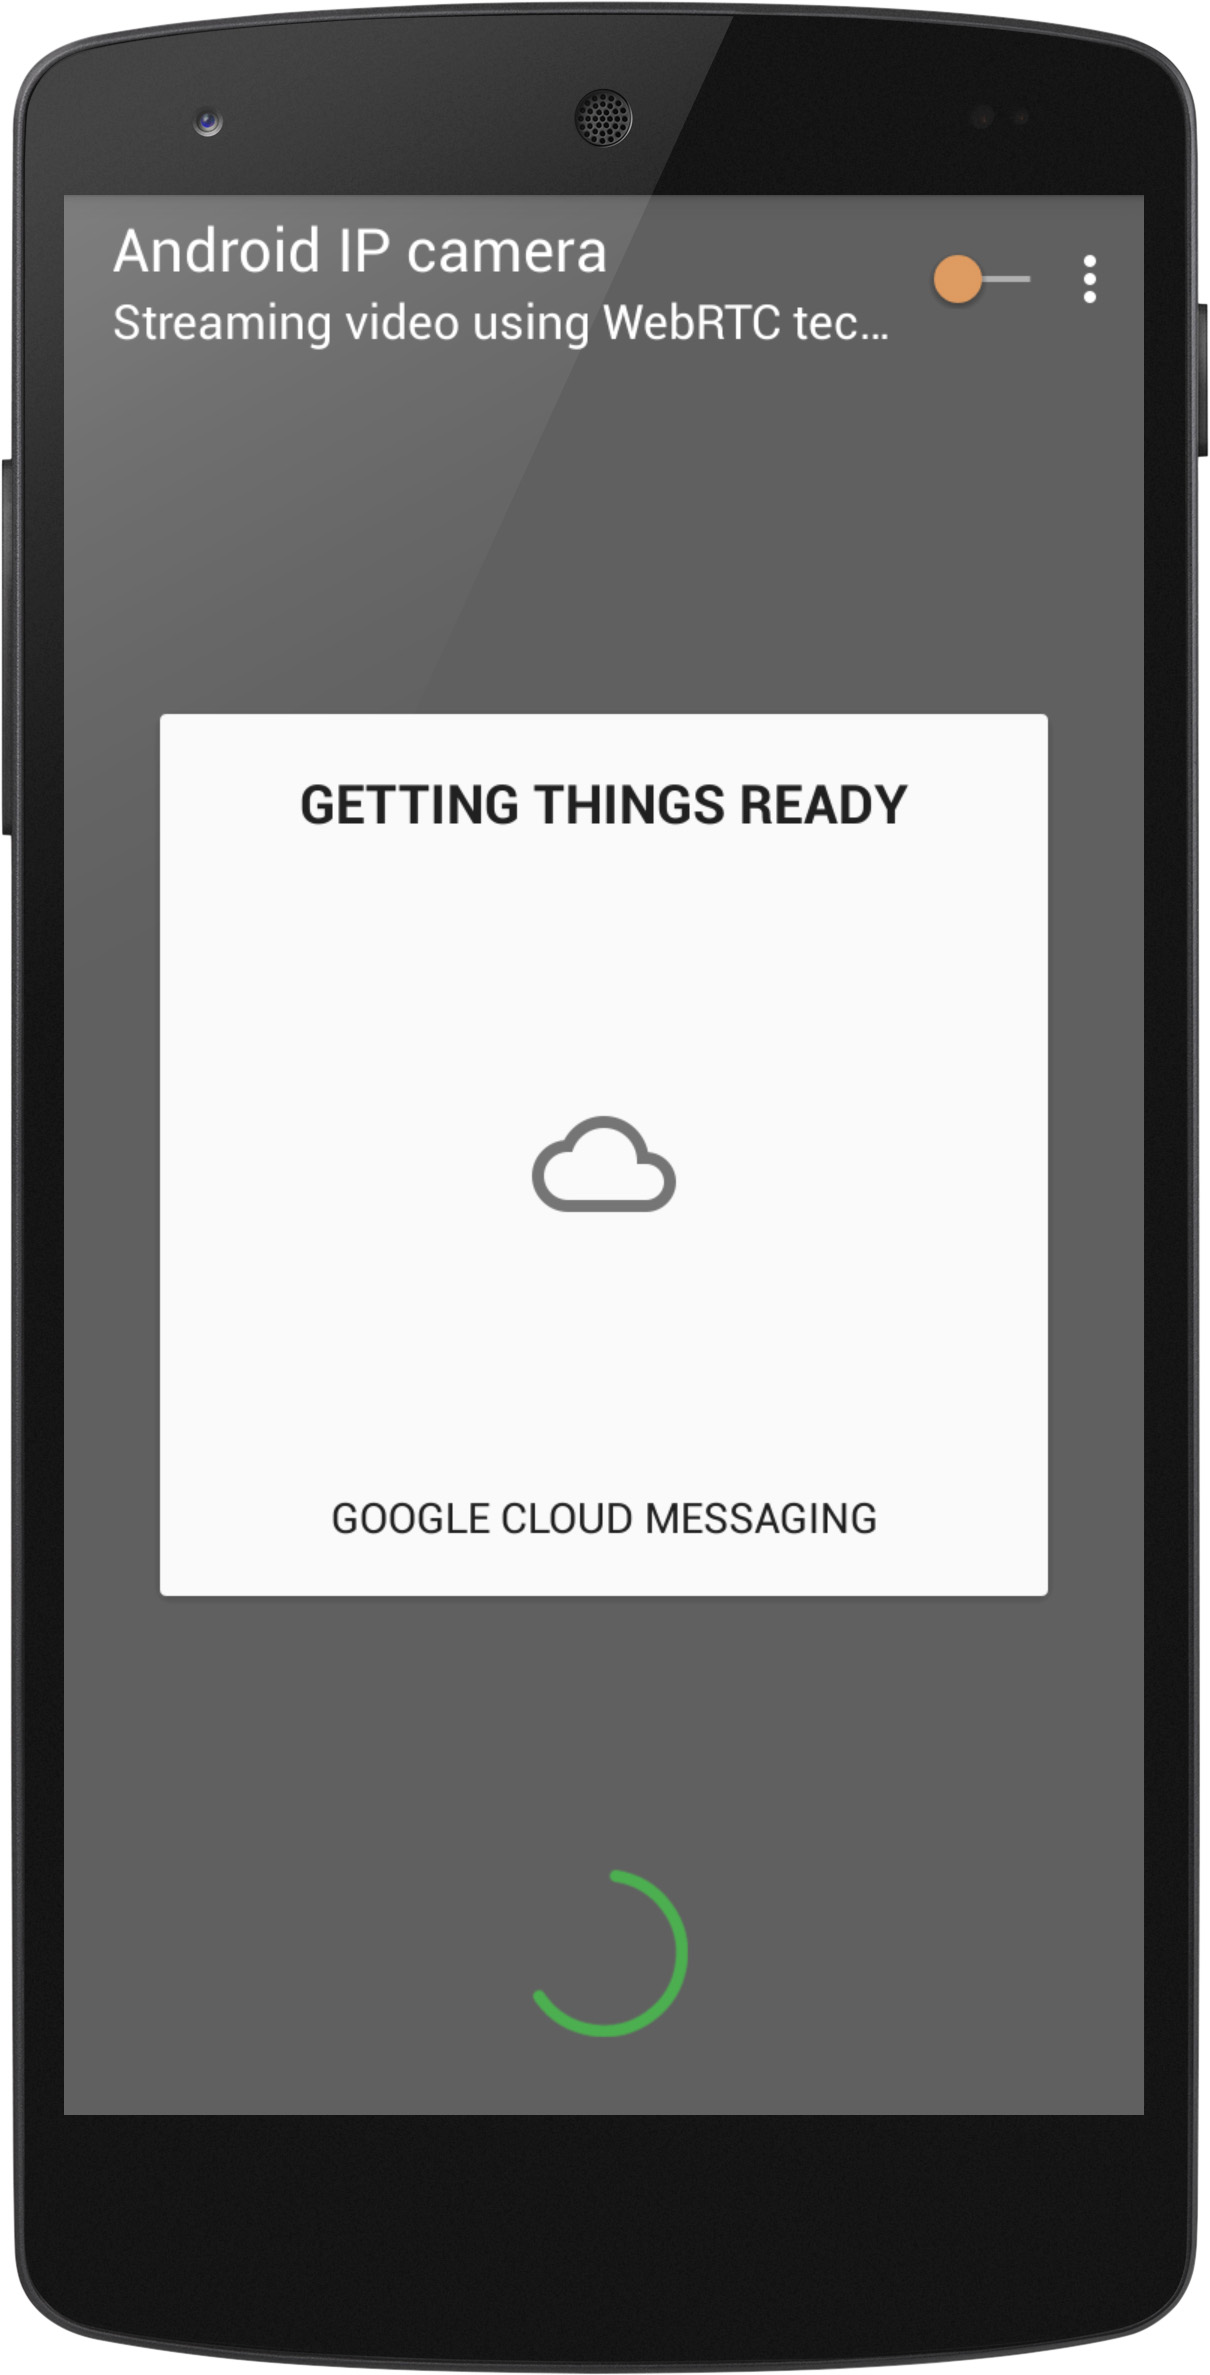
\includegraphics[width=0.24\linewidth]{fig/screenshots/screenshot1_framed.jpg}
	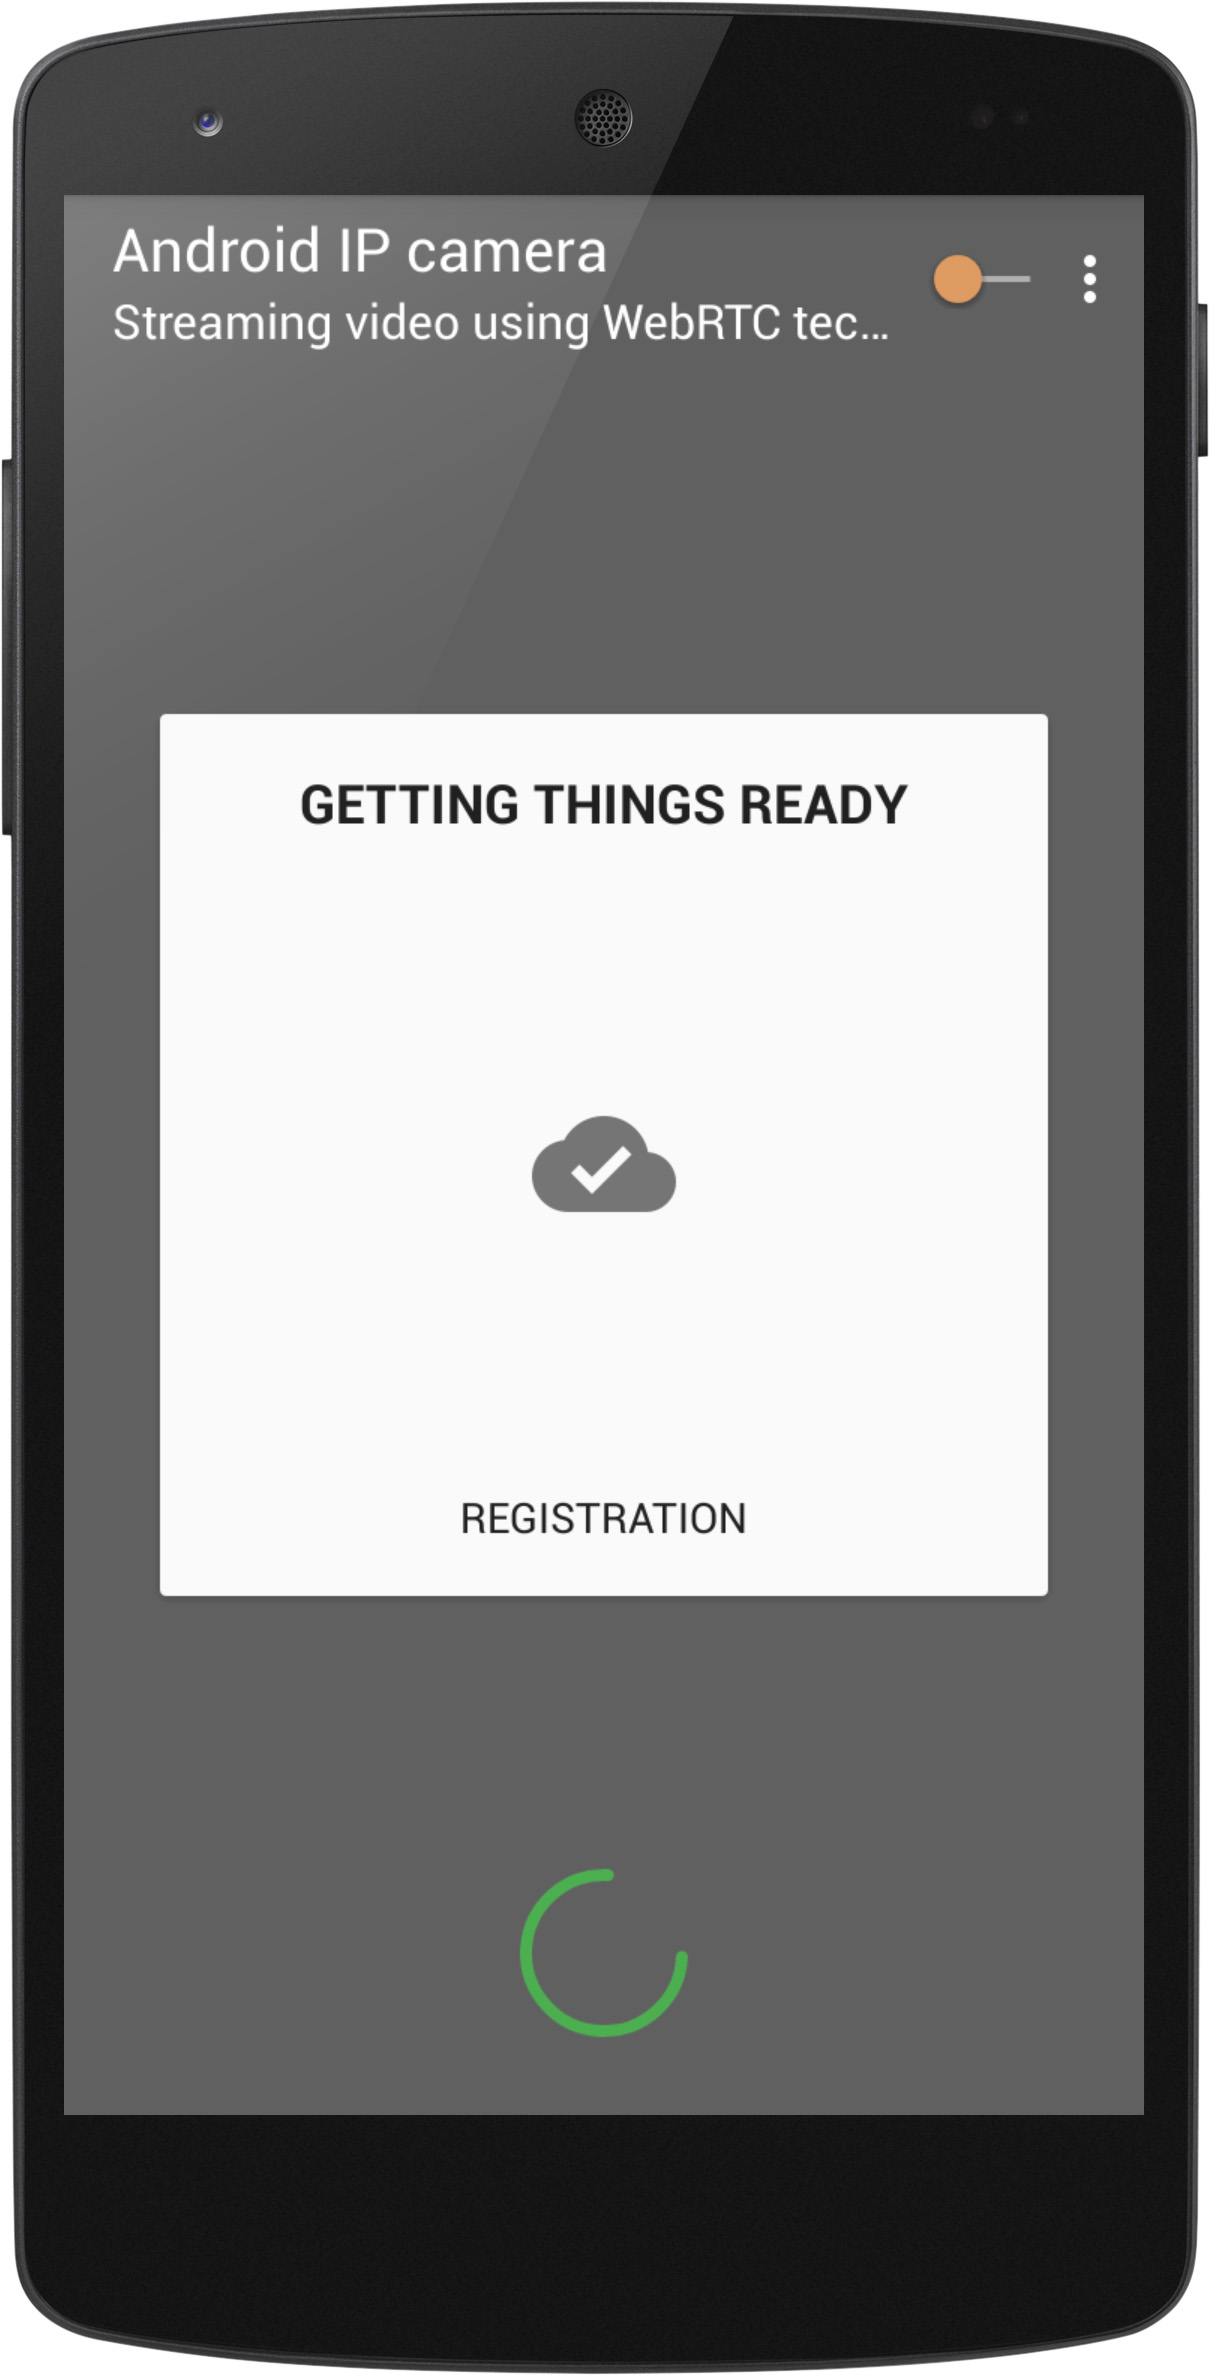
\includegraphics[width=0.24\linewidth]{fig/screenshots/screenshot2_framed.jpg}
	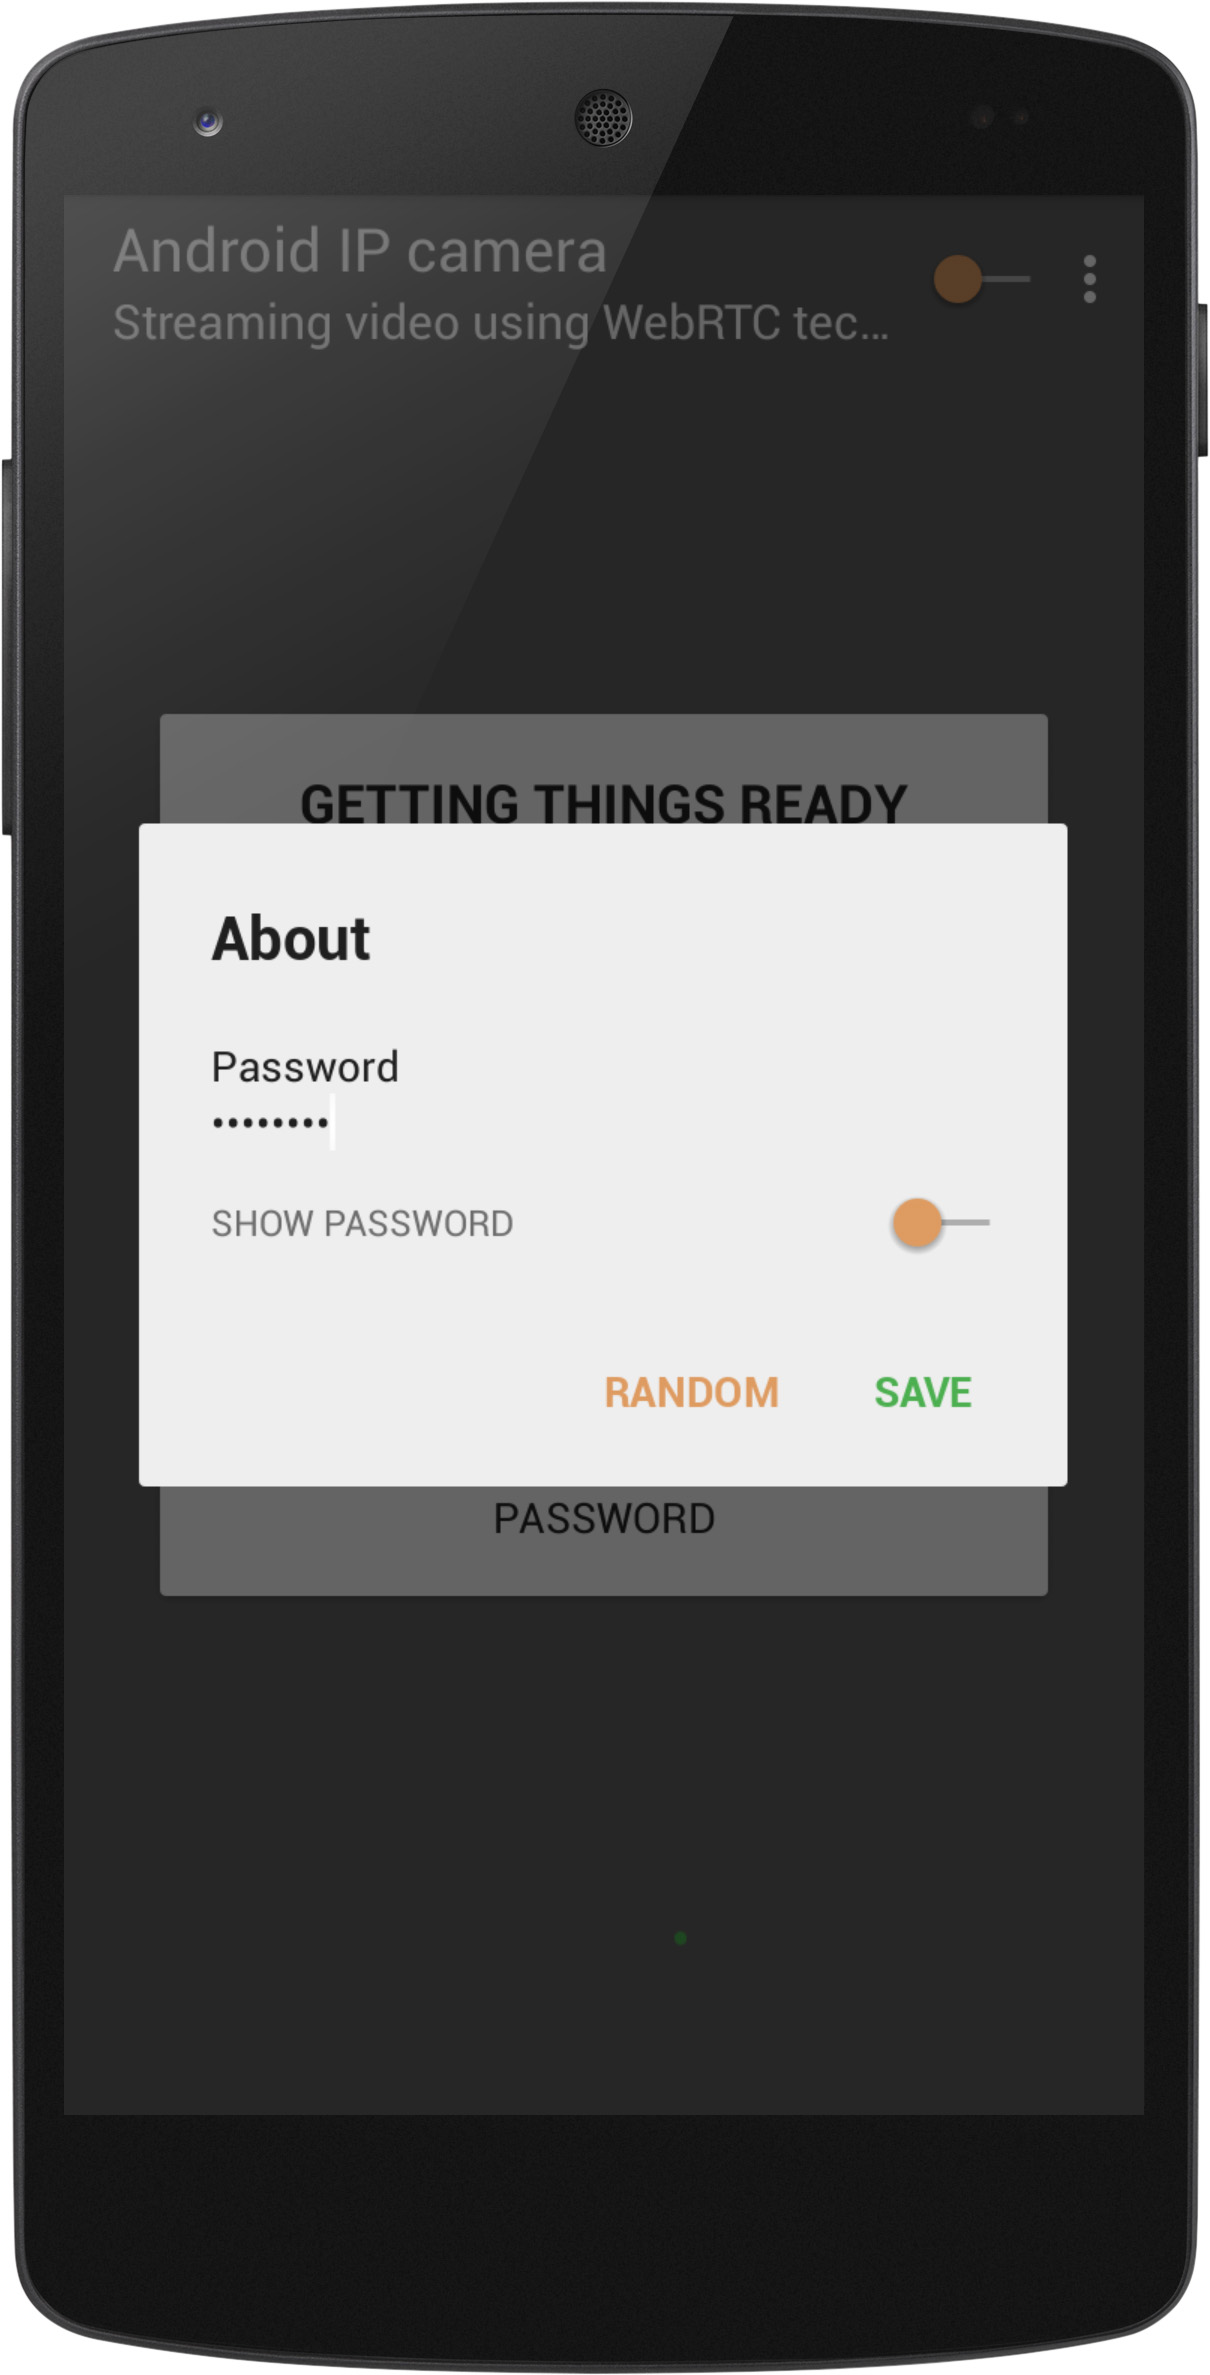
\includegraphics[width=0.24\linewidth]{fig/screenshots/screenshot3_framed.jpg}
	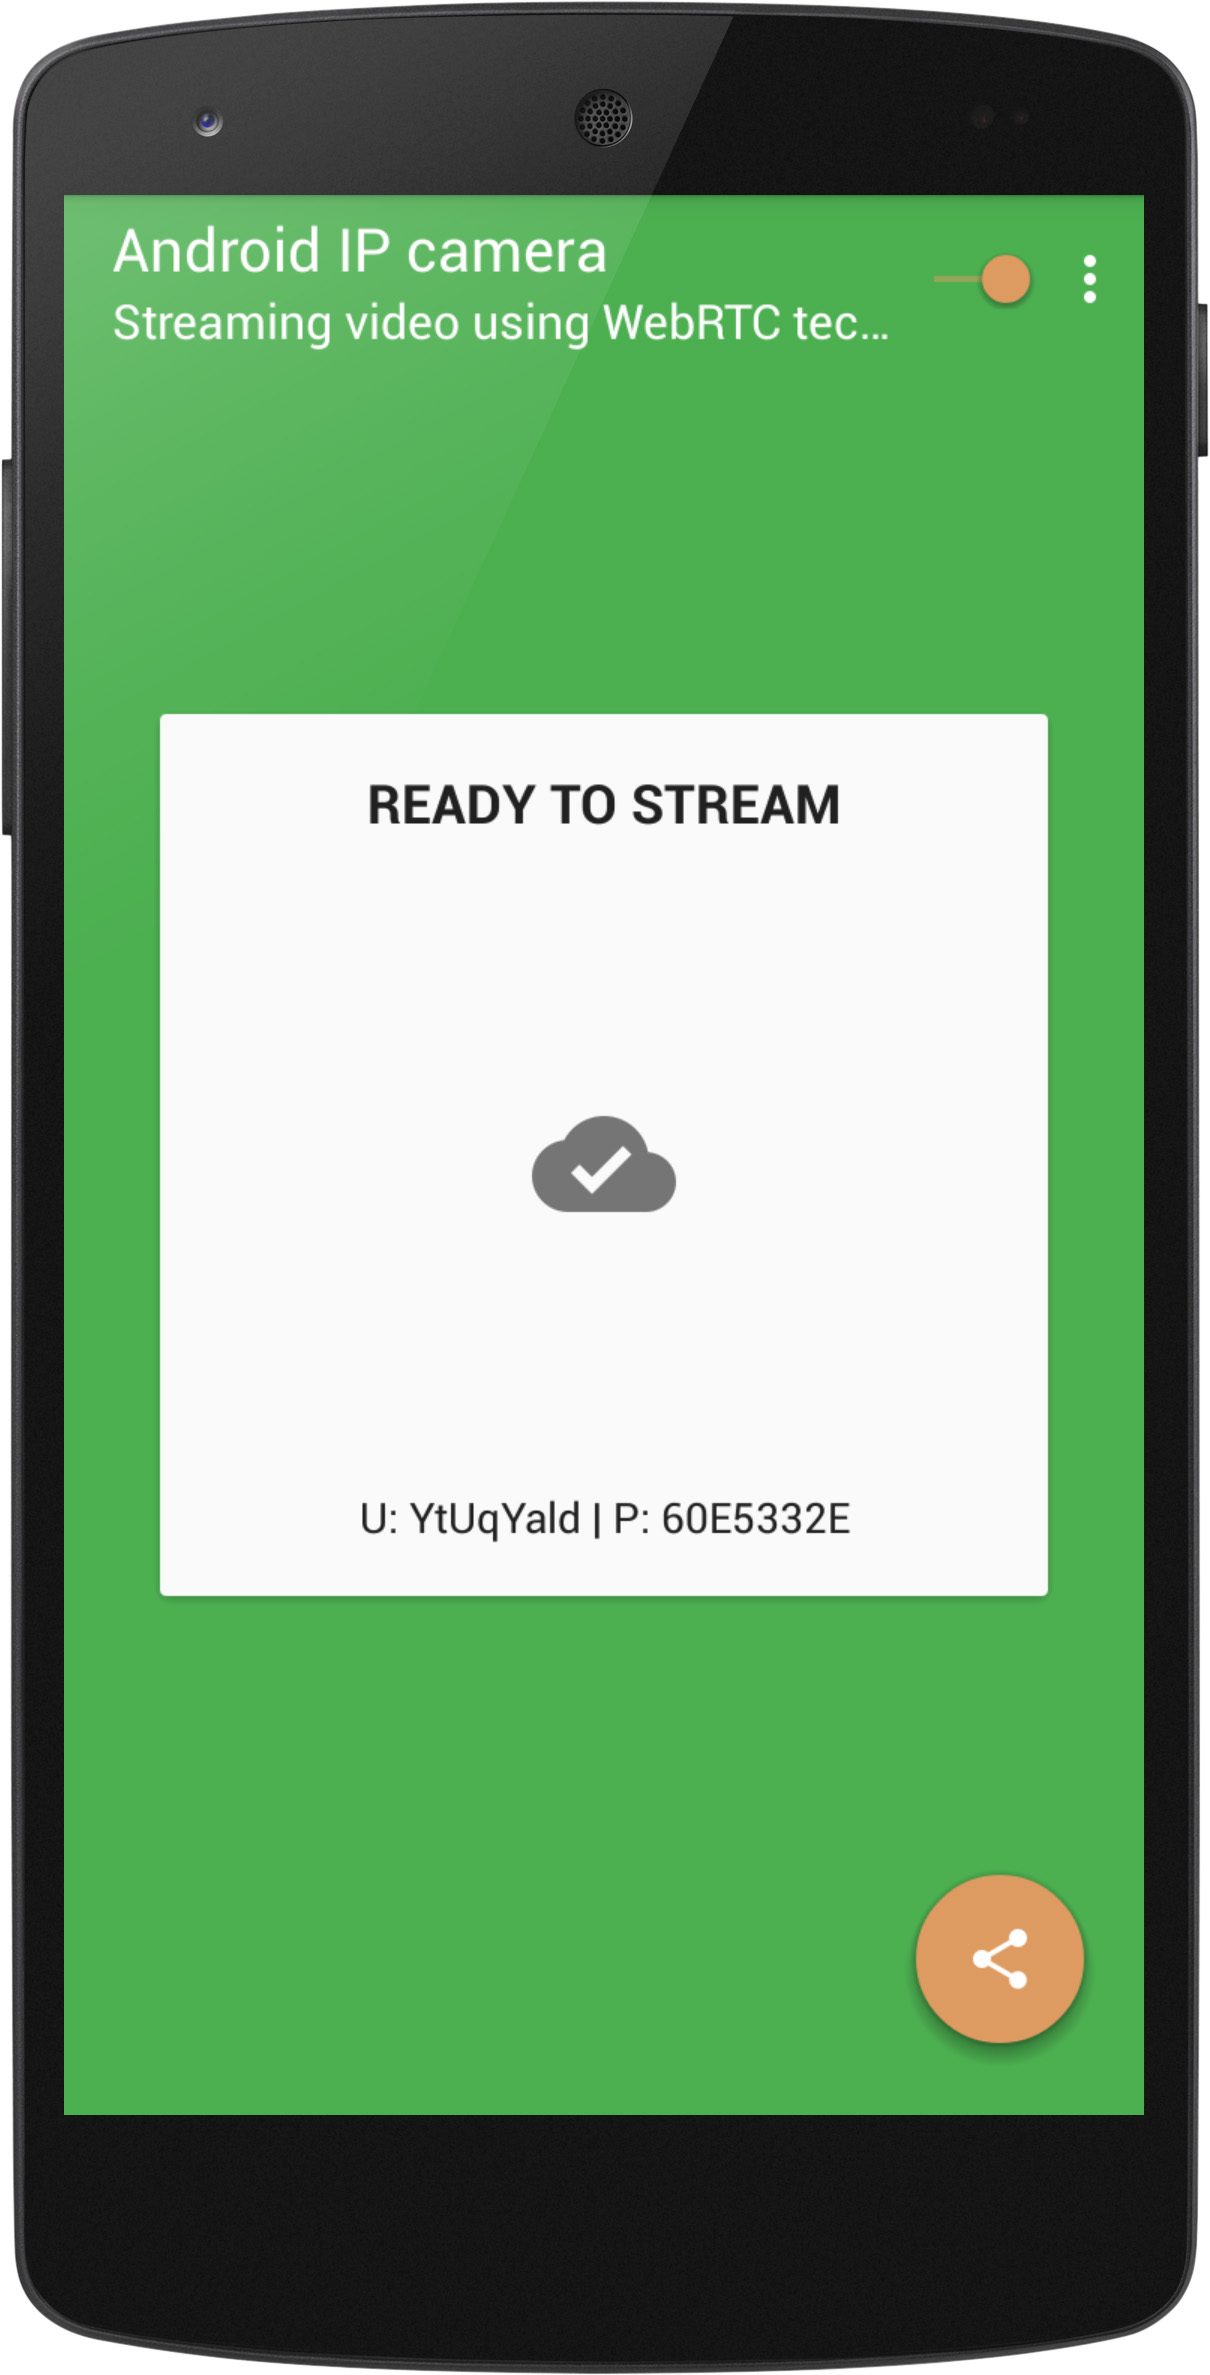
\includegraphics[width=0.24\linewidth]{fig/screenshots/screenshot4_framed.jpg}
	\caption{Screenshots of application's registration process. From left: GCM registration, registration to application server, password setting and ready to stream screen.}
	\label{fig:impl-screenshots1}
\end{figure}


After the registration is completed the user has the possibility to enable the incoming GCM requests for the streaming. This is done with the switch located in Toolbar at the top of each screen, see the last image in figure \ref{fig:impl-screenshots1}. The state of the application is indicated in Card Fragment and also with the background colour which is indicating the state for the first sight.

\begin{figure}[H]
	\centering
	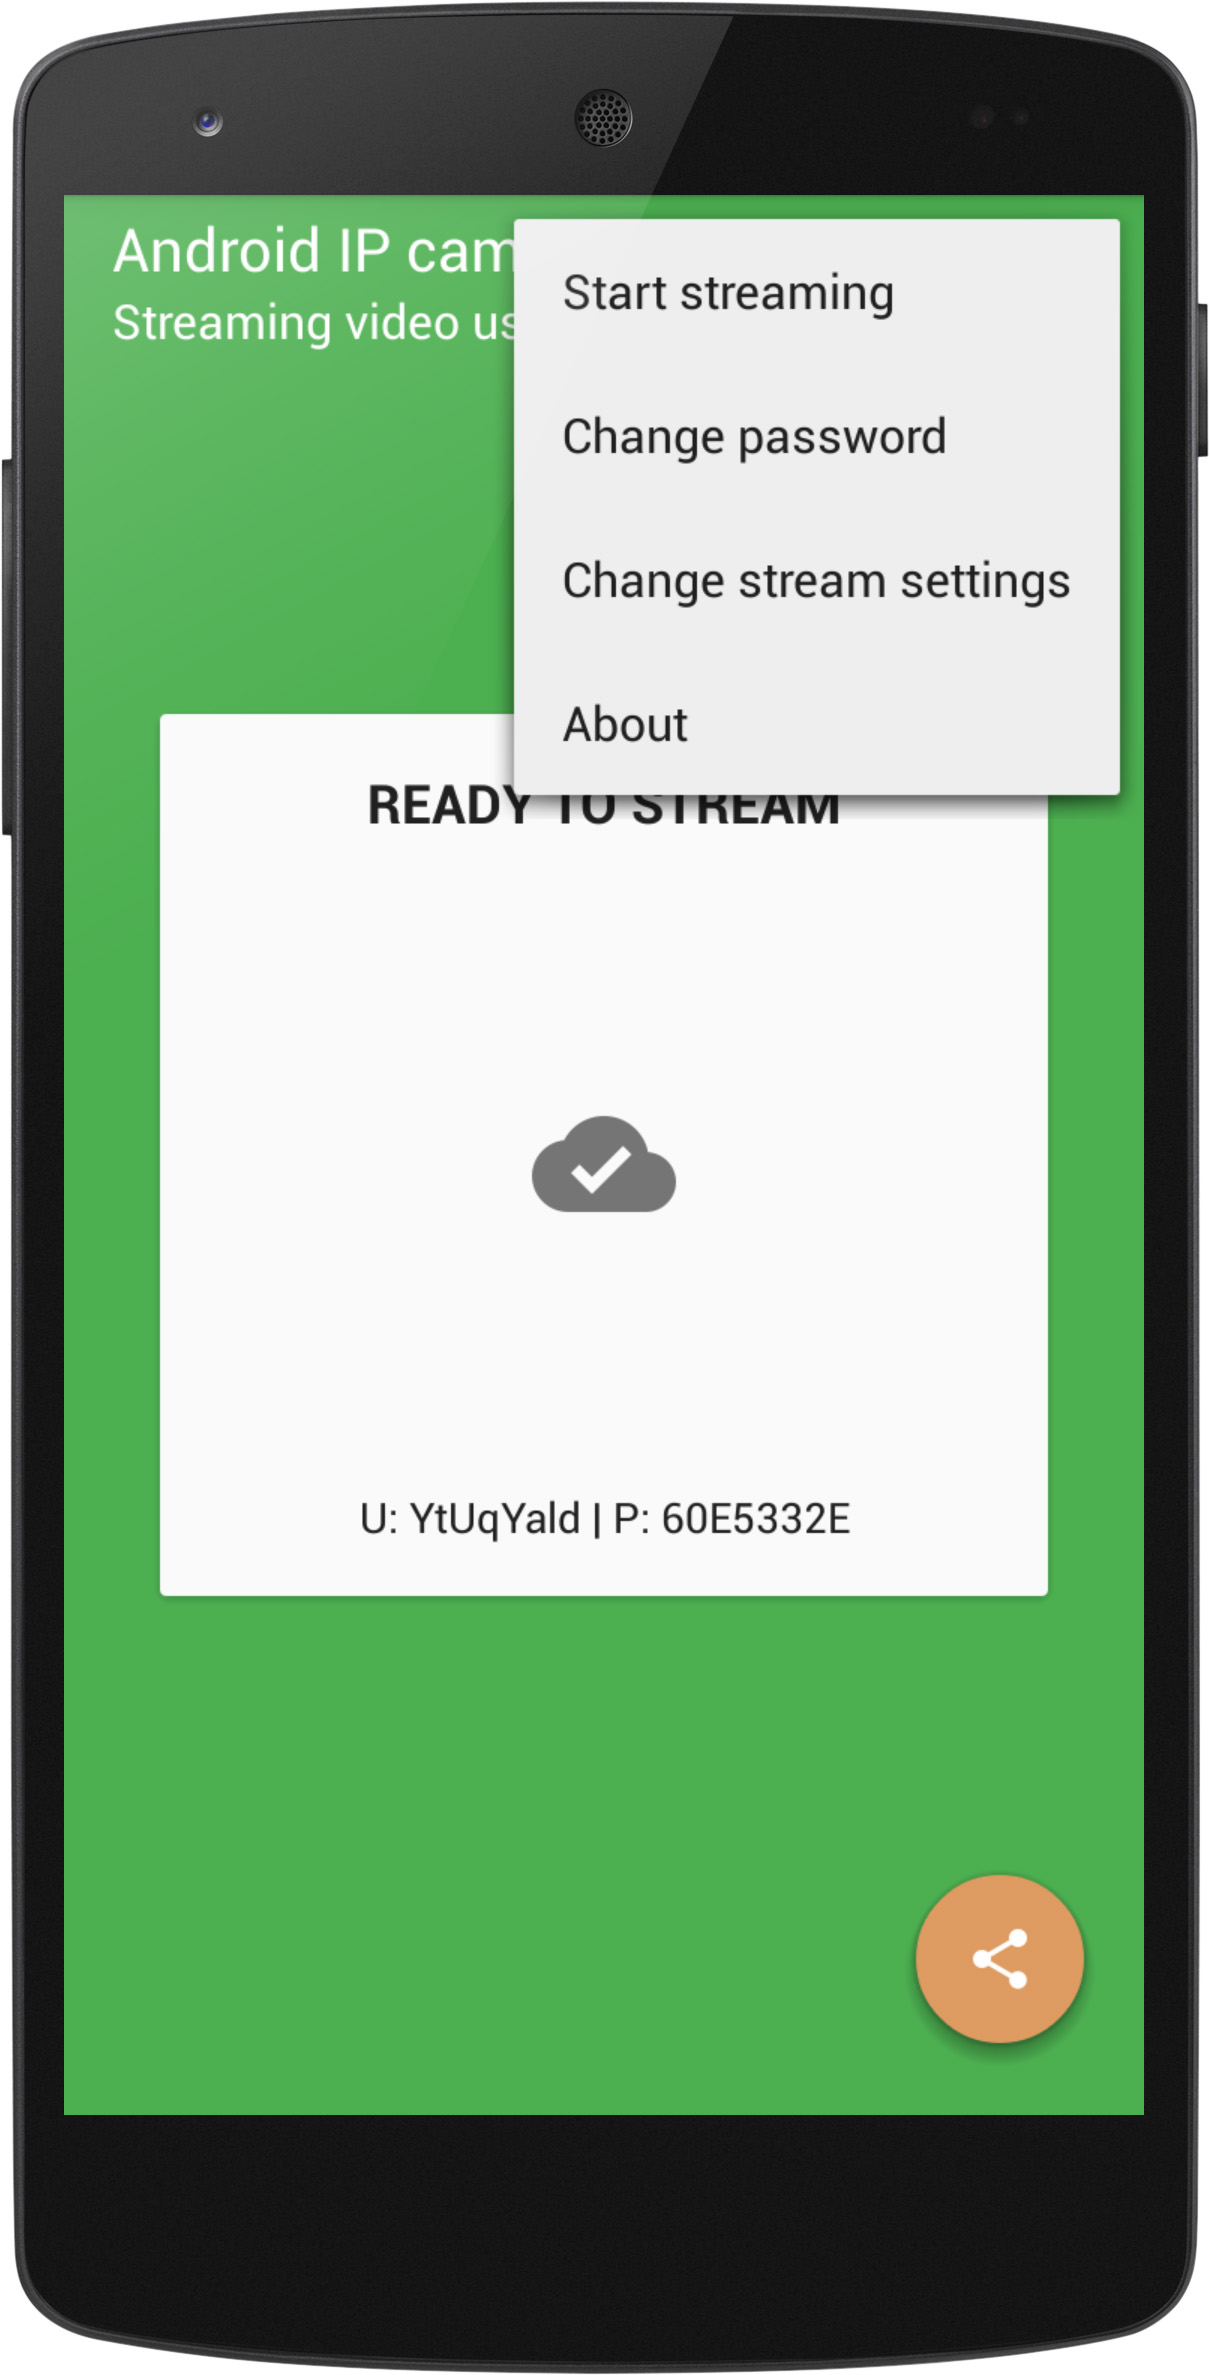
\includegraphics[width=0.24\linewidth]{fig/screenshots/screenshot5_framed.jpg}
	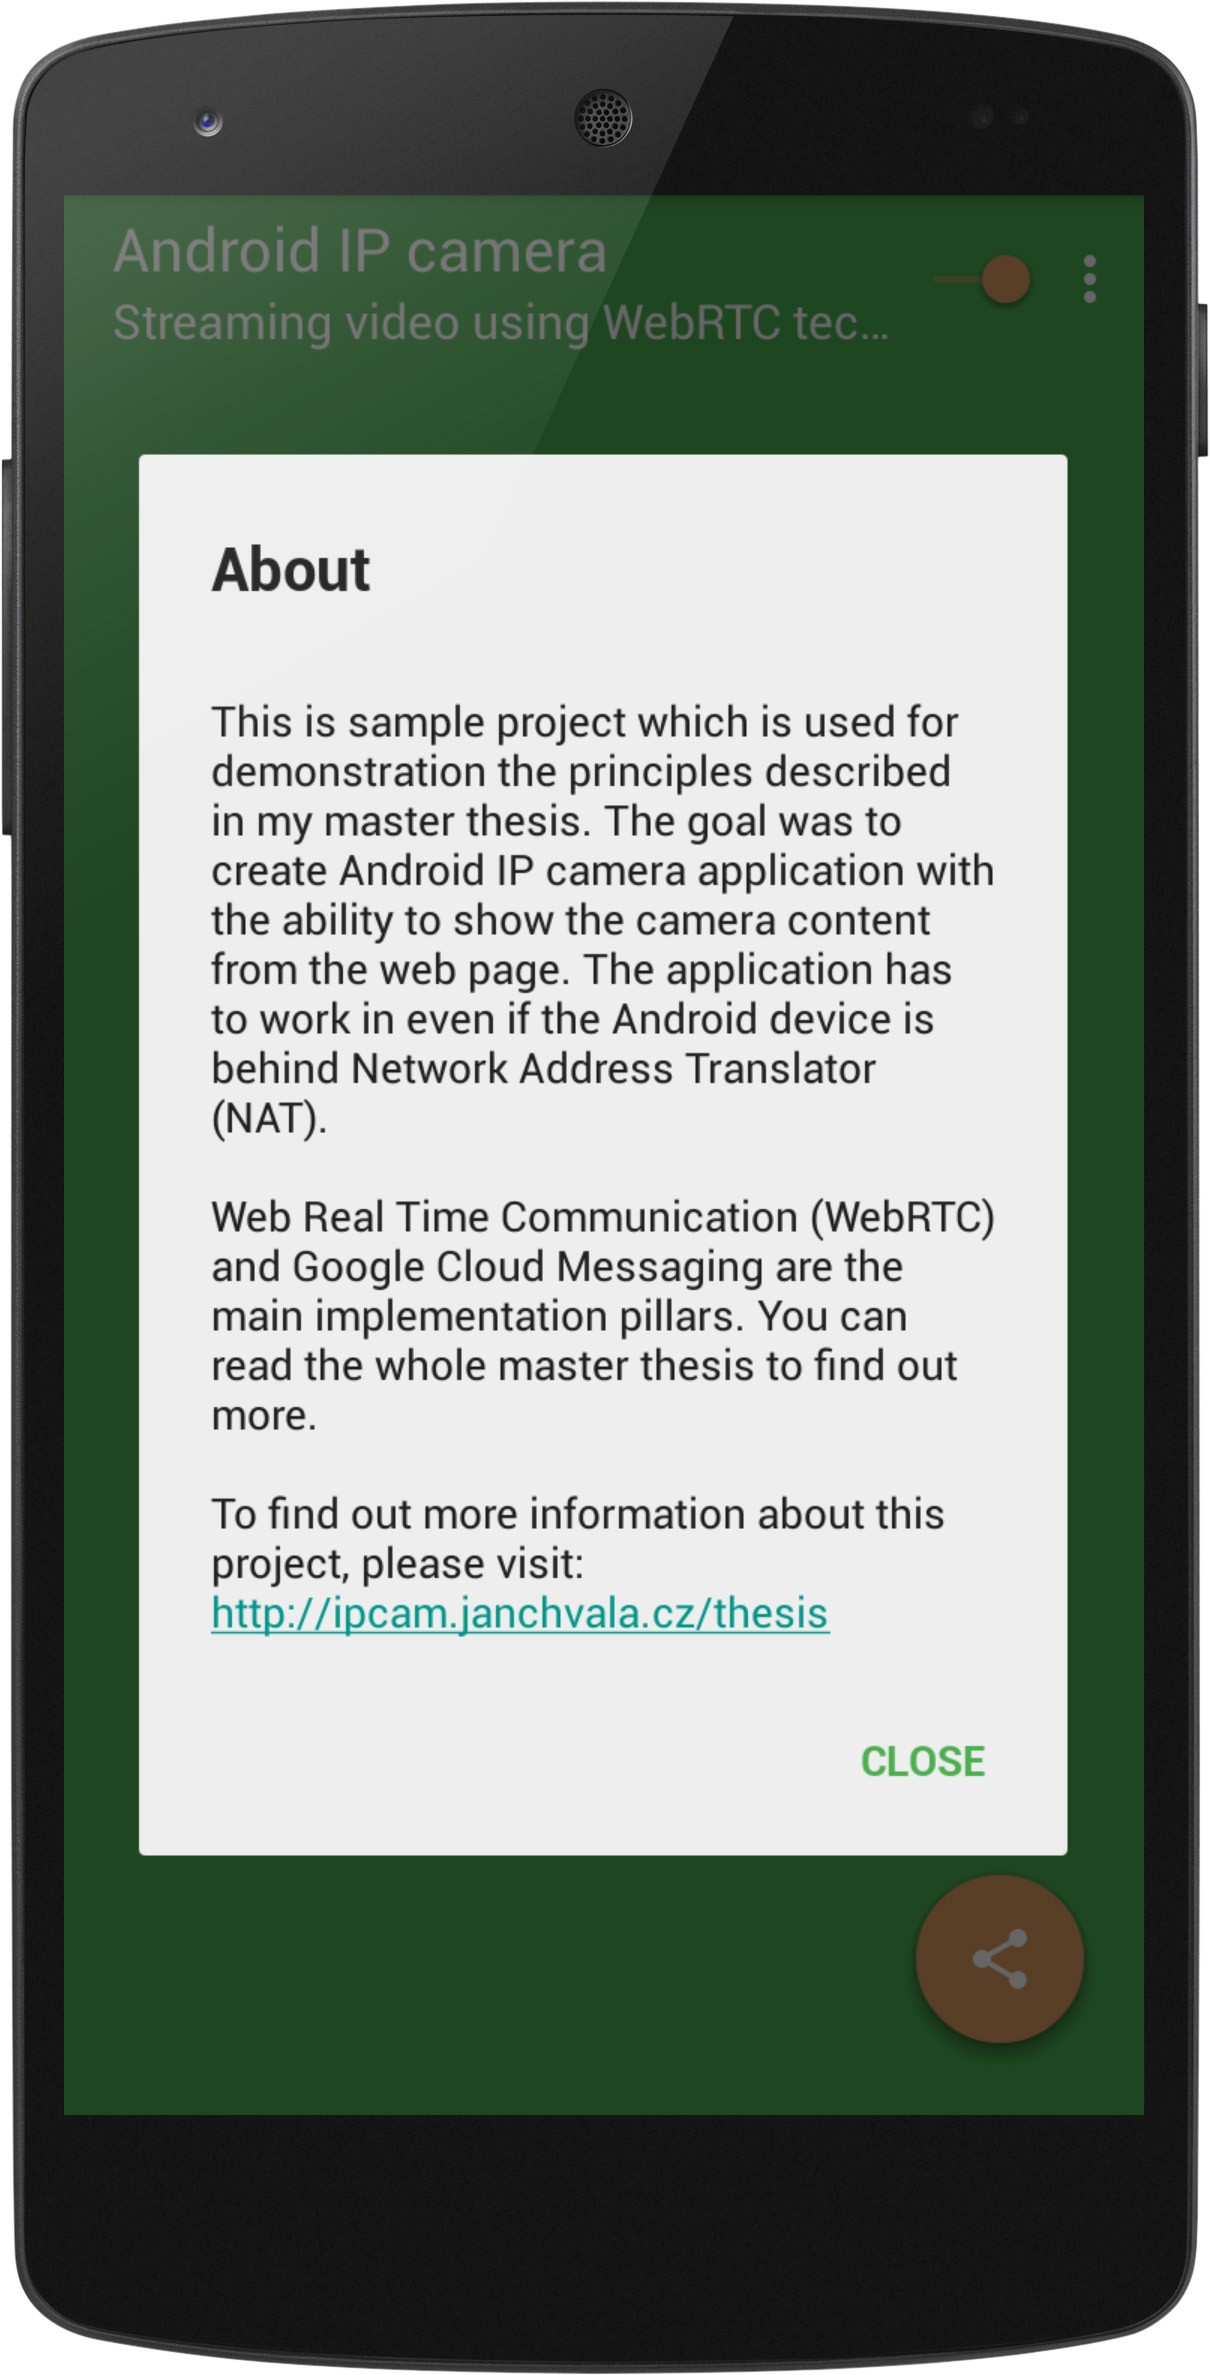
\includegraphics[width=0.24\linewidth]{fig/screenshots/screenshot6_framed.jpg}
	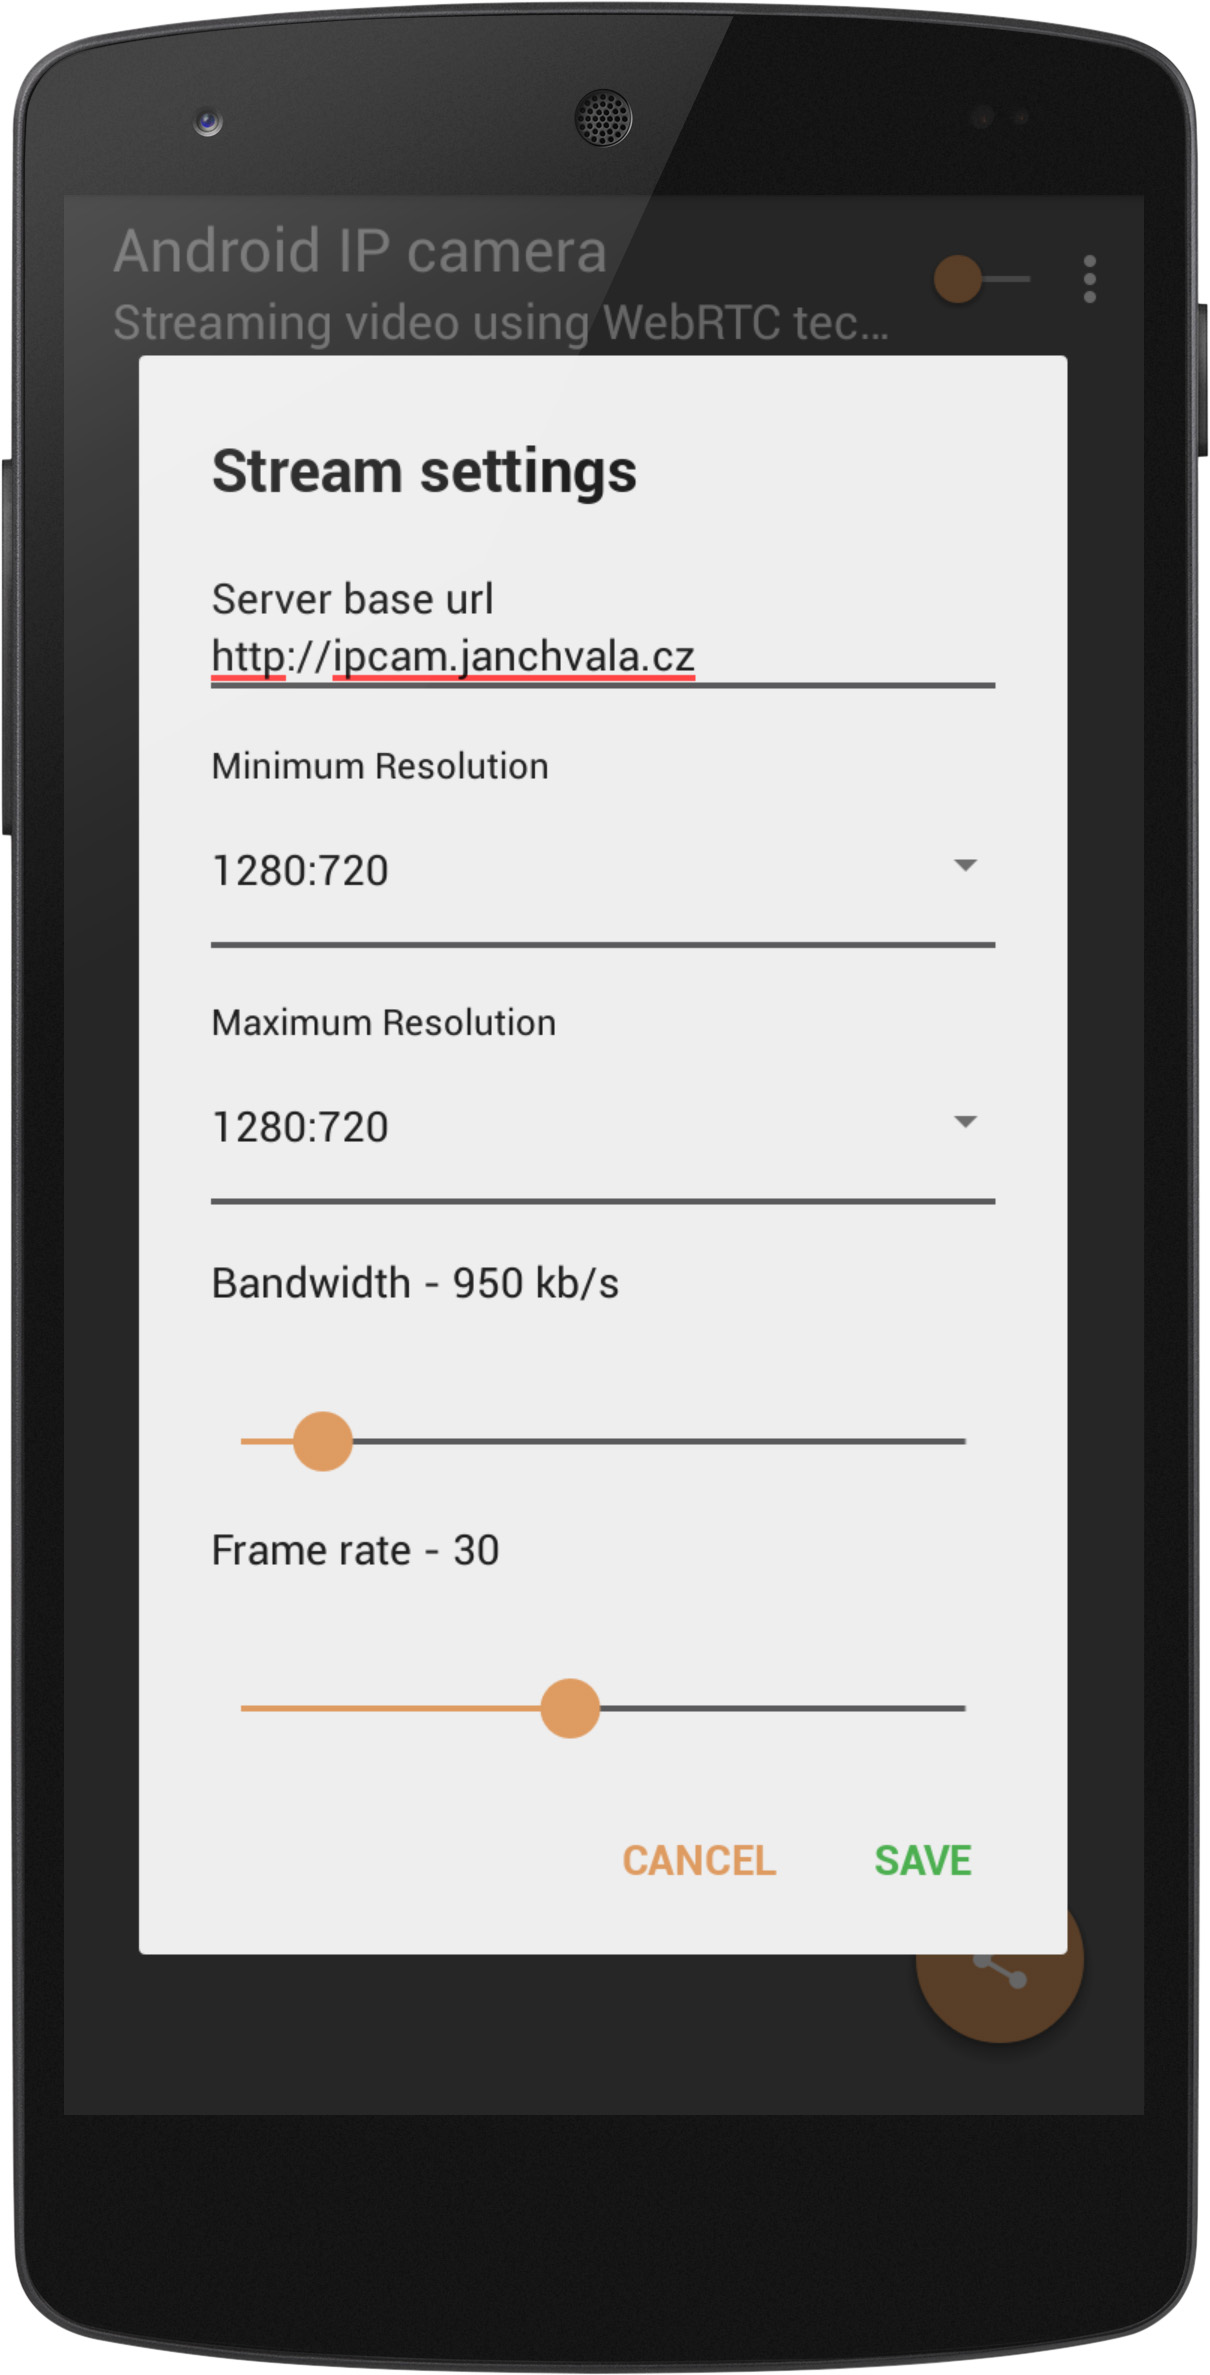
\includegraphics[width=0.24\linewidth]{fig/screenshots/screenshot7_framed.jpg}
	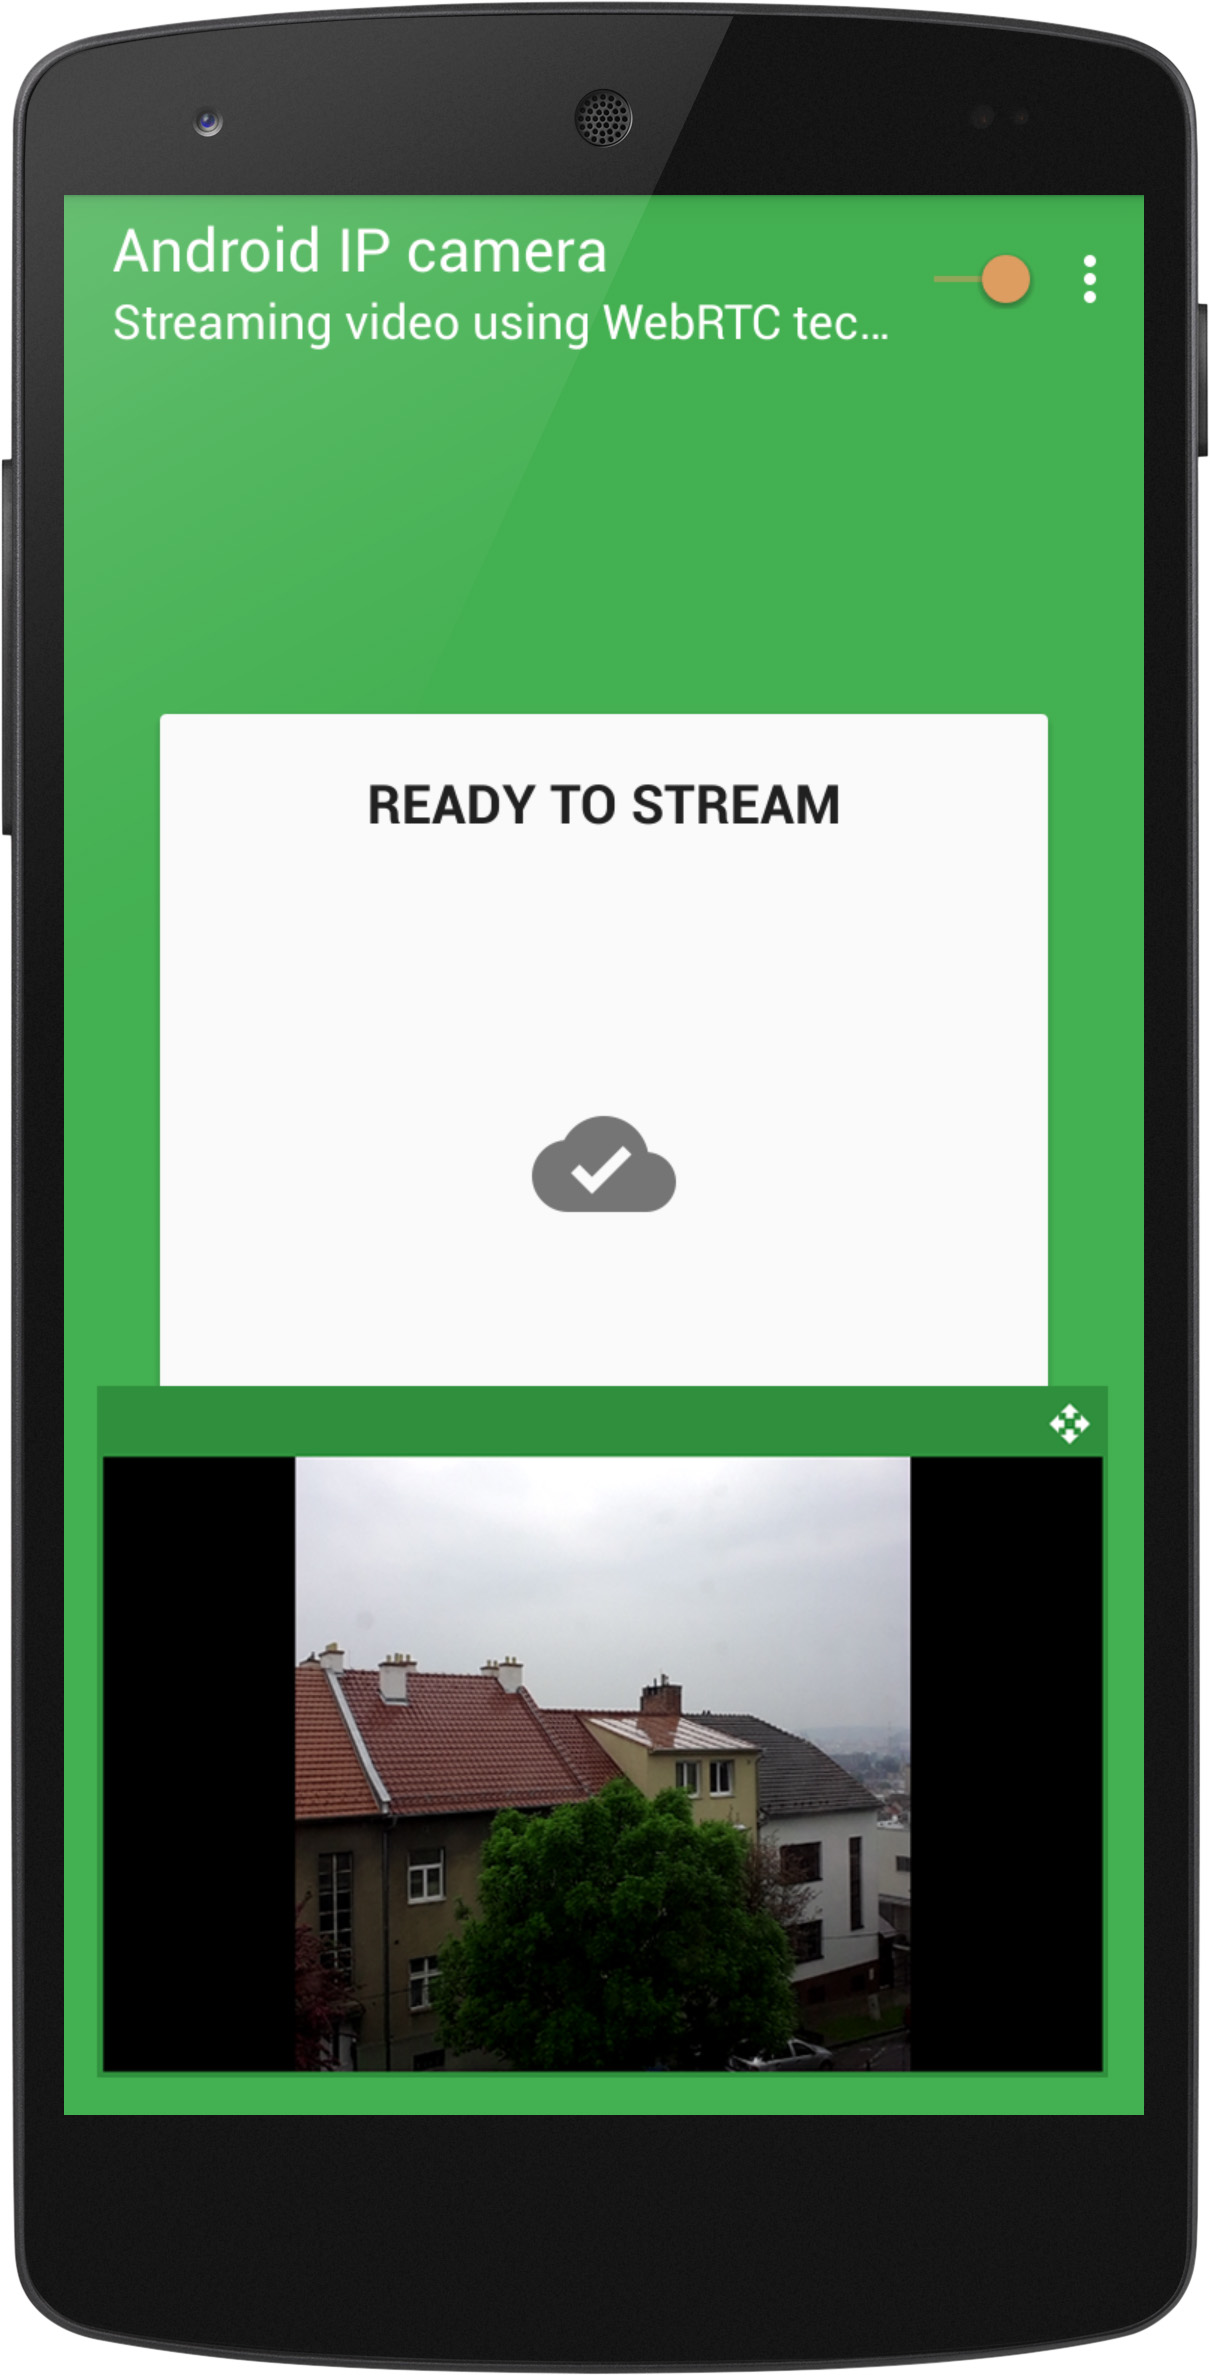
\includegraphics[width=0.24\linewidth]{fig/screenshots/screenshot8_framed.jpg}
	\caption{Screenshots of application during registration process and streaming. Last screenshot also shows streaming notification.}
	\label{fig:impl-screenshots2}
\end{figure}

\newpage
The application provides some actions for the user. Quick action to share the stream URL is accessible from FAB\footnote{Floating Action Button -- circular button introduced in Material design guidelines\\ \url{http://www.google.com/design/spec/components/buttons-floating-action-button.html}} in the left bottom corner of the screen while the others are located in the overflow menu\footnote{Overflow menu is indicated with three vertically aligned dots above each other.}. With these actions the user can easily change the password the same way he initialized it, change stream parameters, start the streaming explicitly or show simple information about the application.

It is also possible to change the server base url which is useful if application url changes. Server registration is reset and new request for streaming code is triggered by changing this option.

Last screen shot shows the notification and also tablet layout user interface. The user has the possibility to stop the streaming or share the streaming URL via notification's buttons. The notification is shown in figure \ref{fig:impl-screenshots3} but it is shown only on Android Lollipop when streaming with native WebView component.

\insertImgHere[1.0]{screenshots/tablet-notification.jpg}{Screenshots of  notification during streaming. Tablet UI.}{fig:impl-screenshots3}

\newpage
\subsection{Handling Google Cloud Messages and streaming}
Google Cloud Messages are processed in three steps in three different parts of the application. The message is invoked the stream is requested by the streaming page \ref{subsec:streaming-page}.

\subsubsection{Receiving messages using BroadcastReceiver}
\textit{GcmBroadcastReceiver} extends \textit{WakefulBroadcastReceiver} which is used to make device awake while receiving messages. It is registered in \textit{AndroidManifest} (\ref{android:manifest}) and it is the first part of the application which is invoked when GCM message is received.

\begin{lstlisting}
@Override
public void onReceive(Context c, Intent intent) {
  // specify that GcmIntentService will handle the intent
  String serviceName = GcmIntentService_.class.getName();
  ComponentName cName = 
    new ComponentName(c.getPackageName(), serviceName); 
  intent.setComponent(cName);

  // Start the service and keep device awake
  startWakefulService(c, intent);

  // set the result of this receive as success
  setResultCode(Activity.RESULT_OK);
}
\end{lstlisting}

\subsubsection{Processing messages using IntentService}
After receiving the message in \textit{BroadcastReceiver} the message is resent to \textit{GcmIntentService} that takes proper action for the message. If it is a real GCM message (not error or deleted event) then the stream is started.
\begin{lstlisting}
@Override
protected void onHandleIntent(Intent intent) {
  Bundle extras = intent.getExtras();
  if (!extras.isEmpty()) { // Initialize GCM
    GoogleCloudMessaging gcm = GoogleCloudMessaging.getInstance(this);

    // getting the message type
    String messageType = gcm.getMessageType(intent);
    // If this is a regular message then start stream
    String mType = GoogleCloudMessaging.MESSAGE_TYPE_MESSAGE;

    if (mType.equals(messageType)) {
      Class wClass = IpCamPreviewWindow_.class;
      Intent i = StandOutWindow.getShowIntent(this,wClass,0);
      startService(i);
    }
  }

  // Releasing the wake lock
  GcmBroadcastReceiver.completeWakefulIntent(intent);
}
\end{lstlisting}

\subsubsection{Starting the stream Service}
Stream is started using \textit{IpCamPreviewWindow\footnote{This window is service with specific UI elements floating above other windows in the system. This is made possible by StandOut library: \url{https://github.com/sherpya/StandOut/}}}. This service creates new \textit{Window} object which can hold UI elements and it is inflated with \textit{WebView}. Then the \textit{WebView} loads streaming page from application server and \textit{WebRTC} takes care about the rest of the streaming. The code below shows the layout inflation and \textit{WebView} initial settings.

\begin{lstlisting}
@Override
public void createAndAttachView(int id, FrameLayout frame) {
  // create a new layout from body.xml
  LayoutInflater inflater = (LayoutInflater) getSystemService(LAYOUT_INFLATER_SERVICE);
  inflater.inflate(R.layout.ipcam_window_layout, frame, true);

  wv = (WebView) frame.findViewById(R.id.web_view_id);
  setupWebView(wv);
}

/**
 * setup WebView JavaScript, ChromeClient and load stream page
 */
protected void setupWebView(WebView wv) {
  WebSettings webSettings = wv.getSettings();
  webSettings.setJavaScriptEnabled(true);
  ...
  wv.setWebChromeClient(new WebChromeClient() {
    @Override
    public void onPermissionRequest(final PermissionRequest request) {
      // handling WebRTC permission request
      dispatchPermissionRequest(request);
    }
  });
  wv.loadUrl(IntentHelpers.getStreamUrl(ipCamPreferences));
}
\end{lstlisting}

\noindent
To see how GCM is registered, see section \ref{ssec:gcm-register}.






%\section{Request to start the stream remotely}
%\blind{1}

%\subsection{Use case}
%\blind{1}
%\todoImg
%\blind{1}

%\subsection{Starting the stream -- client}
%\blind{1}

%\insertImg[0.7]{placeholder.pdf}{Communication when the stream is requested.}{fig:impl-stream-page}

%\subsection{Requesting the playback -- server}
%\blind{1}
%\todoImg
%\blind{1}




\newpage
\section{Security and authentication in demo application}
The authentication and security is not crucial for demonstration of WebRTC technology but it is not desirable to allow anybody to see private streaming.

The application allows to protect device stream with a password which is set up during application first launch on Android device (it can be changed later on). This password is checked on every request from a participant to join created streaming session. The request is then accepted or rejected based on password equality.

\begin{lstlisting}
// set up the password with JavaScript interface from Android
var password = Android.getPassword();

// participant requests access to session
connection.onRequest = function(e) {
  // check if the passwords equal
  if (e.extra.password !== password){
    // the passwords do not match - reject access
    connection.reject(e);
  } else { // accept the request
    connection.accept(e);
  }
};
\end{lstlisting}


There is no protection for the server REST API so anybody who can catch the device code can simply start the stream on the device. We would have to implement user management and registration on the server side to be able to protect it which is out of scope of this thesis. With that in mind the demo application is not intended to be a ready production because of the lack of server REST API protection.

\section{The choice of WebRTC library}
There were more options to choose from when deciding which library to use when working with WebRTC. A few developers try to use the WebRTC and thus they build libraries on top of this edge technology. This section will shortly describe considered libraries and the reasons why they were chosen or not.

\subsection{PeerJS}
The first option found was PeerJS\footnote{PeerJS homepage:\url{http://peerjs.com/}} library. This library is very simple to use and from my point of view it is the easiest to work with. It has very simple API and it also provides the ability to use free \textit{PeerServer} which is responsible for the signalling process.

The main problem is that this library does not support one way video streaming. This is crucial for the resultant application because it is not desirable to request permissions from the user who only wants to play the video stream.

Another problem for me concerning this library is that it seems to be stuck in development. Their master branch on GitHub repository is four months old and it does not seem to be progressing.

\subsection{RTCMultiConnection v2}
Another solution that was the one actually used in the resultant application was the RTCMulticonnection\footnote{RTCMultiConnection homepage: \url{http://www.rtcmulticonnection.org/}} in its version 2.2.2. This library is well documented and allows a lot of customizations. There are also many good examples of working with this library.

The main reason for using this library is that it supports one--way multimedia streaming. This allows to request permission only from the streaming device. It also reduces the data transmission because the session does not contain any empty streams which could affect the bandwidth.

Another good reason is that Muaz Khan (The author of this library) has made it open sourced and he is very actively working on it.

\subsection{RTCMultiConnection v3 beta}
A new version of previously mentioned library was published on 1st April. I was trying to switch the resultant application to use this new version of the RTCMultiConnection library, which provides some more functionality such as build in room protection by password.

It also comes with signalling server build on top of Node.js which is the technology used for the application server. But it is still in beta and there were problems with the signalling process. The problems were making the established connection to fall apart after a couple of seconds of successful stream transmission.

There is a lot of going on around this library and we can be looking forward to seeing its improvements in the near future. I would recommend taking a look at this library for those interested in working with WebRTC.\\
